\section{Scénario 1 : Phase d'initialisation}
\label{sec:scenario1}

Le premier scénario ciblé est la \textbf{phase d'initialisation} de MetaDONE, c'est-à-dire la séquence complète qui s'étend de l'ouverture d'un projet jusqu'à l'état \texttt{PROJECT\_DEFAULT\_REPOSITORY IS OPENED}, tel qu'il apparaît dans les logs (figure~\ref{fig:logs-startup}). Cette phase est exécutée à chaque lancement de l'outil et constitue le premier point de friction perçu par l'utilisateur~: la médiane de nos mesures est de \textbf{18\,198~ms} (min~17\,673 / max~18\,650 ; CV~$=$~1,8\,\%), calculée sur 10 répétitions dans l'environnement décrit à la section~\ref{sec:env} (mesures complètes en annexe~\ref{ann:mesures-s1-a}).

\begin{figure}[h]
\centering
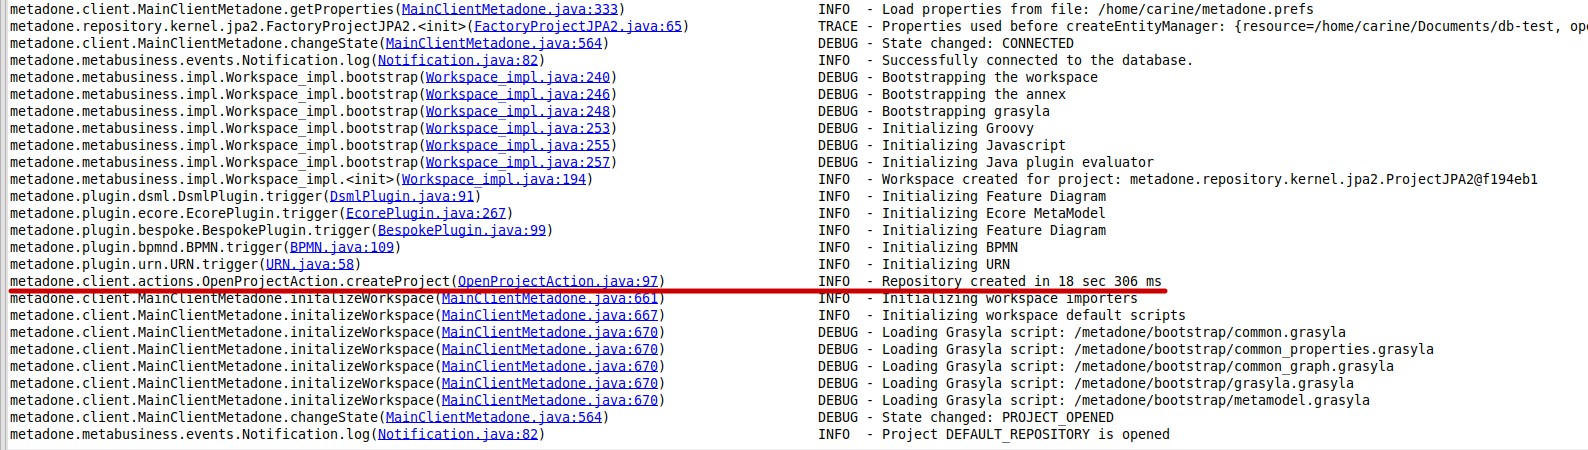
\includegraphics[width=\textwidth]{img/scenario1/ouverture-1.png}
\caption{Séquence de démarrage de MetaDONE. On distingue les trois phases de bootstrapping (\texttt{workspace}, \texttt{annex},
\texttt{grasyla}) ainsi que l'initialisation des plugins.}
\label{fig:logs-startup}
\end{figure}

Les logs révèlent une séquence structurée en plusieurs étapes distinctes, dont la compréhension est indispensable pour interpréter les résultats
de profilage.

La séquence débute par la connexion à la base de données (\texttt{FactoryProjectJPA2.<init>}) et l'initialisation du gestionnaire JPA (\texttt{createEntityManager}). Vient ensuite le \textbf{bootstrapping},
qui construit en mémoire le graphe réflexif de MetaL$_1$ et MetaL$_2$ à partir de zéro~: il crée les items séminaux (\texttt{Bootstrapping the workspace}), puis le méta-méta-modèle Omega et les types primitifs (\texttt{Bootstrapping the annex}), et enfin charge les scripts GraSyLa de base (\texttt{Bootstrapping grasyla}). Ces trois sous-phases opèrent dans \texttt{Workspace\_impl.bootstrap()} du bundle \texttt{metadone\_bundle\_metabusiness}.

Une fois le \texttt{Workspace} créé, les \textbf{plugins OSGi} sont déclenchés séquentiellement via leur méthode \texttt{trigger()}. Les logs montrent l'initialisation de \texttt{EcoreMetaModel}, \texttt{FeatureDiagram} (déclenché indépendamment par \texttt{DsmlPlugin} puis par \texttt{BespokePlugin}), \texttt{BPMN} et \texttt{URN}.

Enfin, le workspace charge les scripts GraSyLa applicatifs (\texttt{common.grasyla}, \texttt{common\_properties.grasyla}, etc.) via
\texttt{MainClientMetadone.initializeWorkspace()}, avant d'atteindre l'état
\texttt{PROJECT DEFAULT\_REPOSITORY IS OPENED}.

\subsection{Identification des goulots d'étranglement}
\label{sec:scenario1-profil1}

Cette phase d'analyse vise à isoler précisément les sections du code
responsables d'une consommation excessive de ressources. Comme présenté à
la section~\ref{sec:env}, JFR et async-profiler sont deux outils
complémentaires~: JFR fournit une vue structurée des événements JVM sur
l'ensemble de la durée de démarrage, tandis qu'async-profiler localise
précisément les méthodes dominantes via un échantillonnage non biaisé par
le mécanisme de safepoint~\cite{mytkowicz2010evaluating}.

% -----------------------------------------------
\subsubsection{Profilage avec Java Flight Recorder}
% -----------------------------------------------

L'activation de JFR au lancement de la JVM utilise les arguments suivants~:

\begin{verbatim}
-XX:+UnlockCommercialFeatures
-XX:+FlightRecorder
-XX:StartFlightRecording=name=metadone_jfr,settings=profile,
    dumponexit=true,filename=metadone.jfr
-XX:FlightRecorderOptions=stackdepth=256
\end{verbatim}

L'option \texttt{settings=profile} active le profil de collecte étendu,
qui enregistre davantage d'événements au prix d'un surcoût légèrement
supérieur au profil \texttt{default} (environ 2\% contre 1\% selon la
documentation Oracle~\cite{jfr2021oracle}). L'option \texttt{stackdepth=256} augmente la profondeur de pile enregistrée au-delà de la valeur par défaut de 64, ce qui est nécessaire ici~: l'architecture en couches de MetaDONE (\texttt{client} $\to$ \texttt{metabusiness} $\to$ \texttt{repository}, voir chapitre~\ref{chap:architecture}) génère des piles d'appels profondes où les méthodes de bas niveau (bundle \texttt{repository}) ne seraient potentiellement pas visibles avec la valeur par défaut.

L'analyse du JFR via Java Mission Control a mis en évidence un point de congestion majeur~: la méthode \texttt{pcGetdeleted}, qui représente 9,11\% des échantillons CPU de l'ensemble de la session (figure~\ref{fig:jfr-1}).

\begin{figure}[h]
\centering
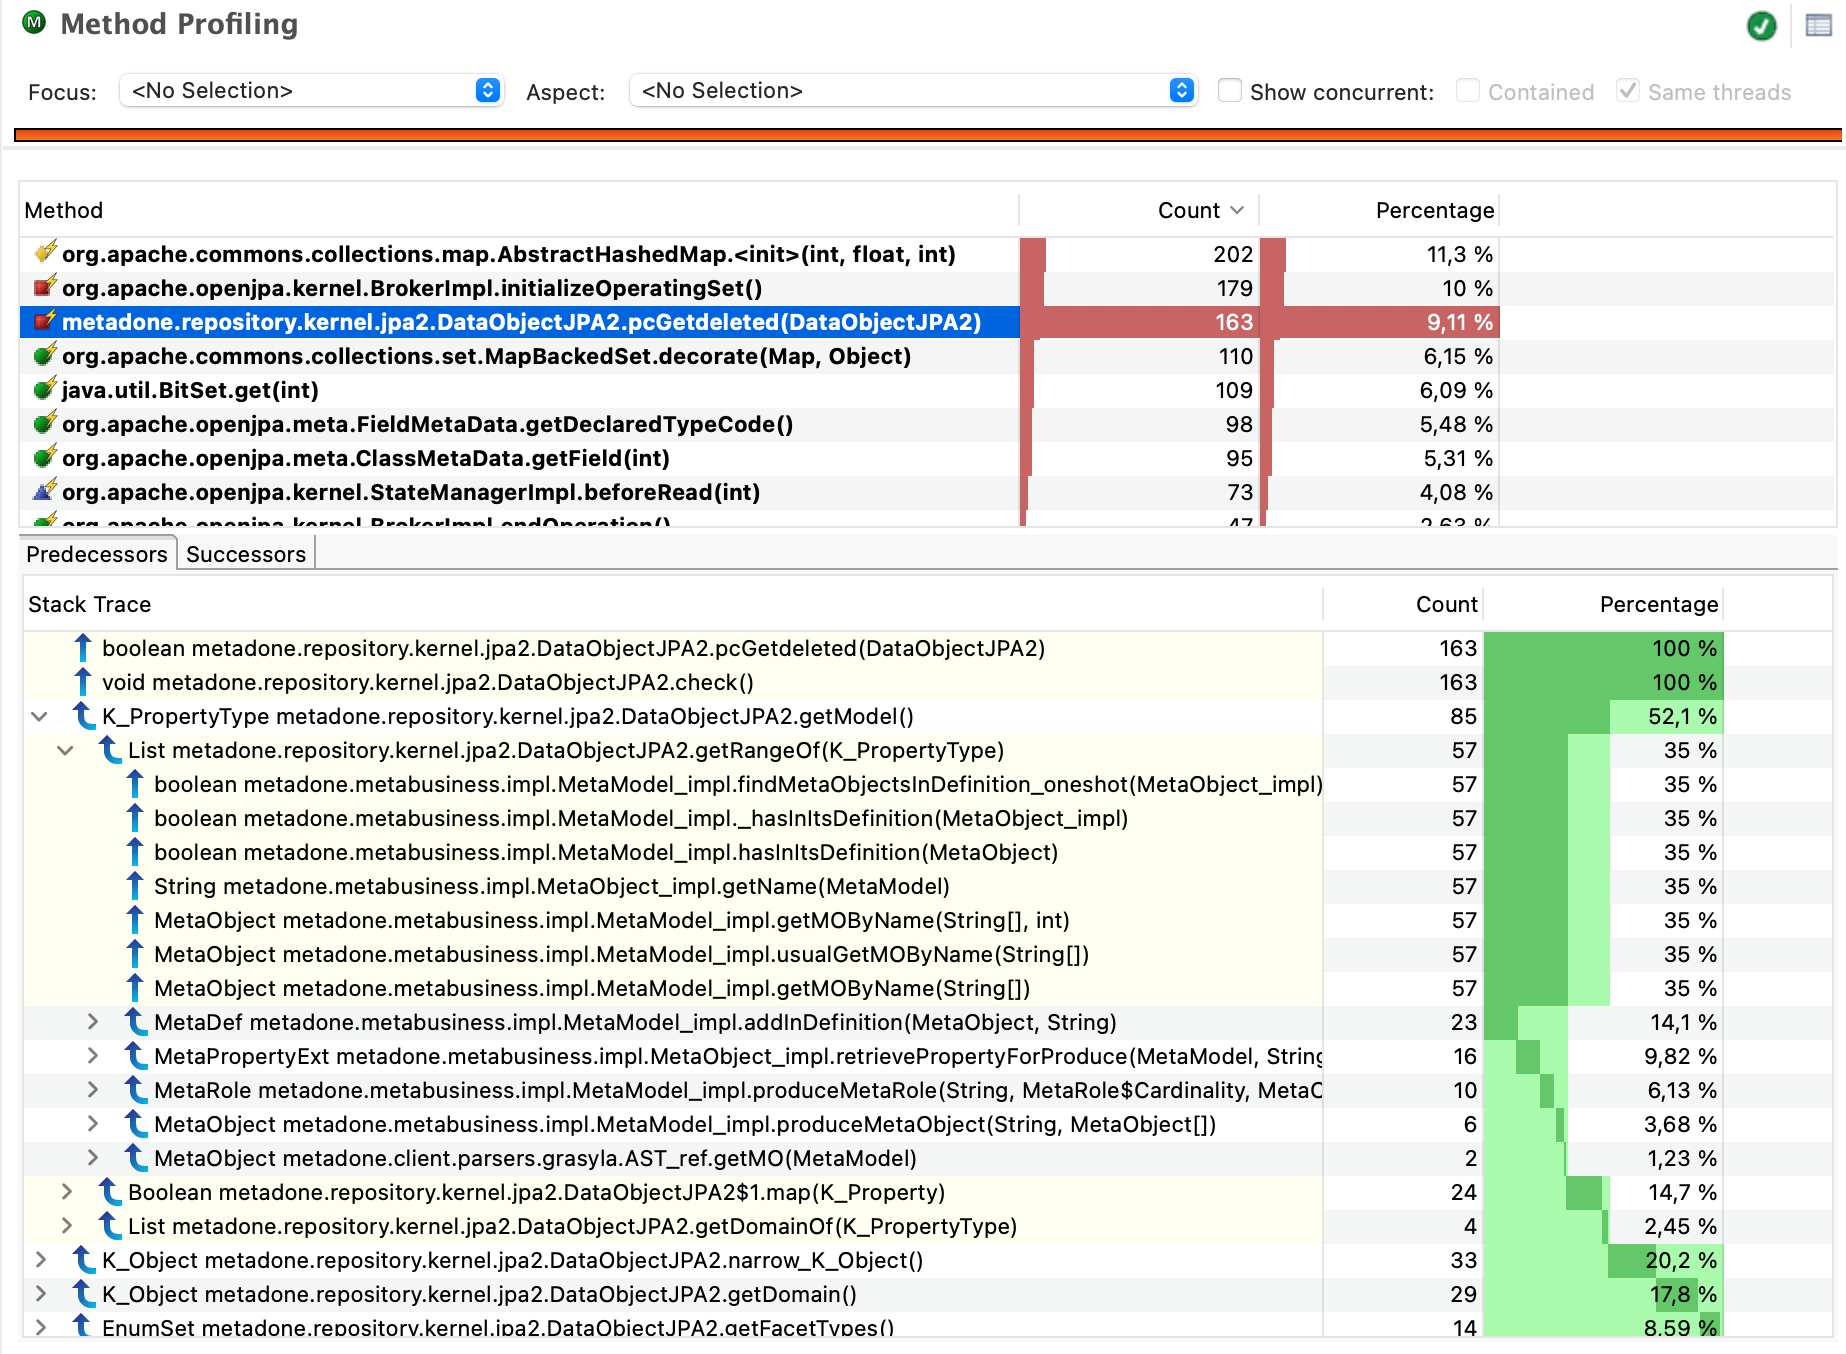
\includegraphics[width=0.8\textwidth]{img/scenario1/jfr-1.png}
\caption{Java Mission Control --- Method Profiling. La méthode
\texttt{pcGetdeleted} (bundle \texttt{metadone\_bundle\_repository\_jpa2})
domine avec 9,11\% des échantillons.}
\label{fig:jfr-1}
\end{figure}

La remontée des prédécesseurs dans JMC reconstruit la \textbf{chaîne
d'appels critique}~:

\begin{center}
\texttt{pcGetdeleted} $\leftarrow$
\texttt{check} $\leftarrow$ 
\texttt{getModel} $\leftarrow$
\texttt{getRangeOf} $\leftarrow$ 
\texttt{findMetaObjectsInDefinition\_oneshot} $\leftarrow$
\texttt{\_hasInItsDefinition} $\leftarrow$
\texttt{hasInItsDefinition} $\leftarrow$
\texttt{...}
\end{center}

Les quatre premières méthodes appartiennent à la couche repository et les suivantes à la couche metabusiness. Avant
d'en analyser le code, nous utilisons async-profiler pour valider et
affiner ce diagnostic.

% -----------------------------------------------
\subsubsection{Analyse approfondie via flamegraph}
% -----------------------------------------------

Async-profiler est lancé en parallèle de JFR selon la configuration
décrite à la section~\ref{sec:env}. Le flamegraph global
(figure~\ref{fig:prof1-flame1}) offre une vue d'ensemble de la répartition
du CPU sur l'ensemble de la phase de démarrage.

\begin{wrapfigure}{r}{5.5cm}
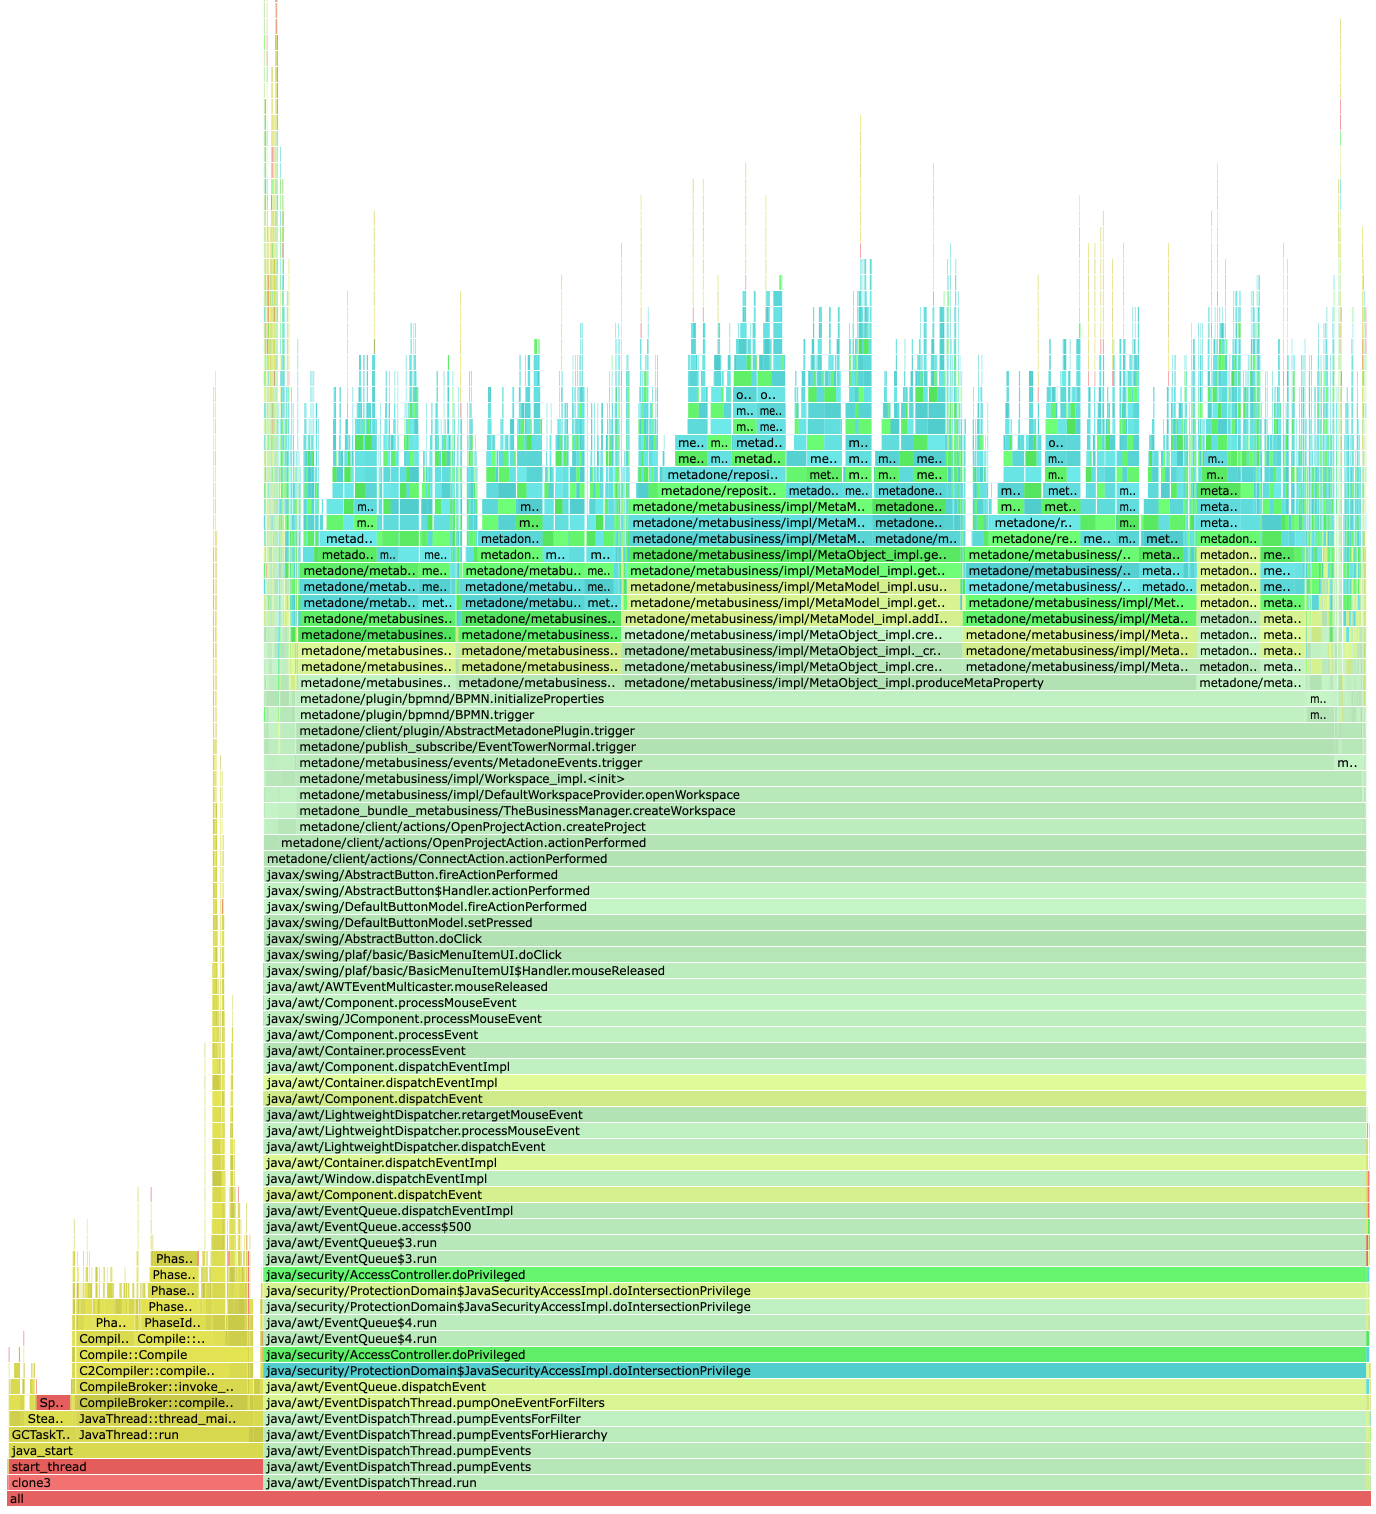
\includegraphics[width=5.5cm]{img/scenario1/prof1/flame1.png}
\caption{Flamegraph global de la phase d'initialisation.}
\label{fig:prof1-flame1}
\end{wrapfigure}

Rappelons la lecture d'un flamegraph~: l'axe vertical représente la
profondeur de pile --- plus on monte, plus on s'approche de la méthode
terminale effectivement exécutée. L'axe horizontal, trié alphabétiquement,
représente le temps CPU total passé dans chaque méthode et ses appelées~:
un rectangle large signale un hotspot.

En se concentrant sur les méthodes identifiées par JFR, les pourcentages
d'occupation CPU lors du démarrage sont les suivants~:

\begin{itemize}
    \item \texttt{pcGetdeleted} --- 35,97\%
    \item \texttt{check} --- 38,48\%
    \item \texttt{getModel} --- 35,79\%
    \item \texttt{getRangeOf} --- 29,33\%
    \item \texttt{findMetaObjectsInDefinition\_oneshot} --- 56,44\%
    \item \texttt{\_hasInItsDefinition} --- 56,57\%
    \item ...
\end{itemize}

Ces pourcentages correspondent à la proportion des échantillons CPU dans
lesquels la méthode apparaît dans la pile d'appels. La divergence entre
les 9,11\% rapportés par JFR et les 35--56\% du flamegraph s'explique par
leur différence de portée~: JFR mesure sur la totalité de la session
(y compris les phases I/O et d'attente JVM), tandis qu'async-profiler isole
ici la phase de création du repository.

Pour plus de clarté, les graphes de la figure~\ref{fig:prof1-zoom} isolent la phase d’initialisation du plugin BPMN. Celui-ci constitue le principal goulot d’étranglement, tant par sa durée de chargement que par la densité de ses appels.

\begin{figure}[htbp]
\begin{subfigure}{\textwidth}
    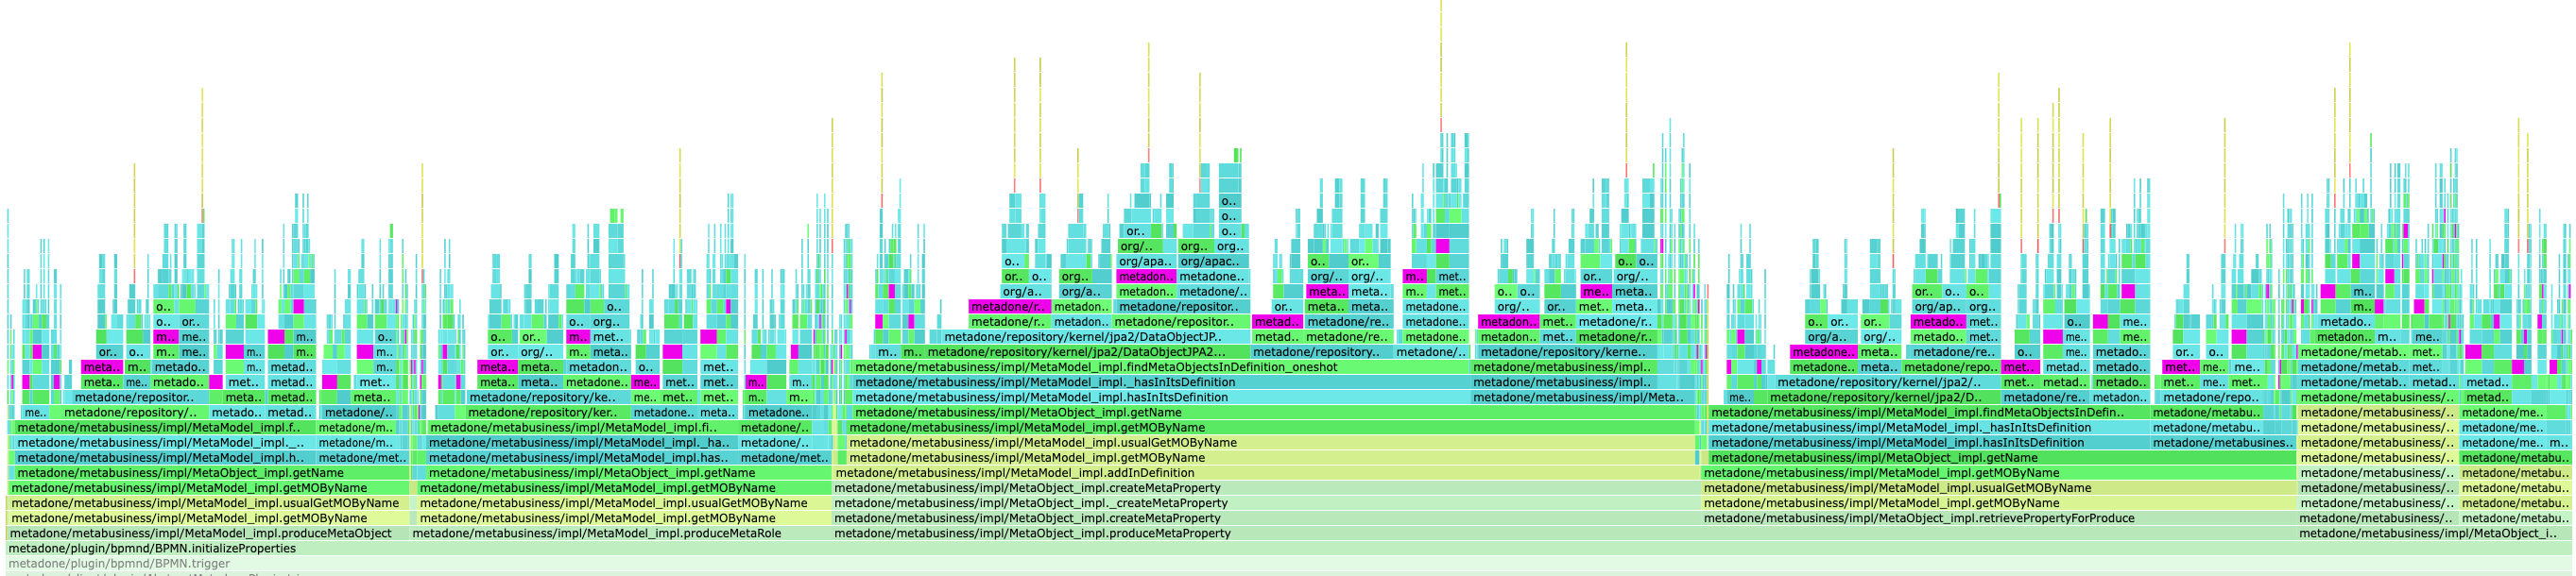
\includegraphics[width=\textwidth]{img/scenario1/prof1/pcGetdeleted.png}
    \caption{\texttt{pcGetdeleted} ---
    bundle \texttt{metadone\_bundle\_repository\_jpa2}}
\end{subfigure}

\medskip
\begin{subfigure}{\textwidth}
    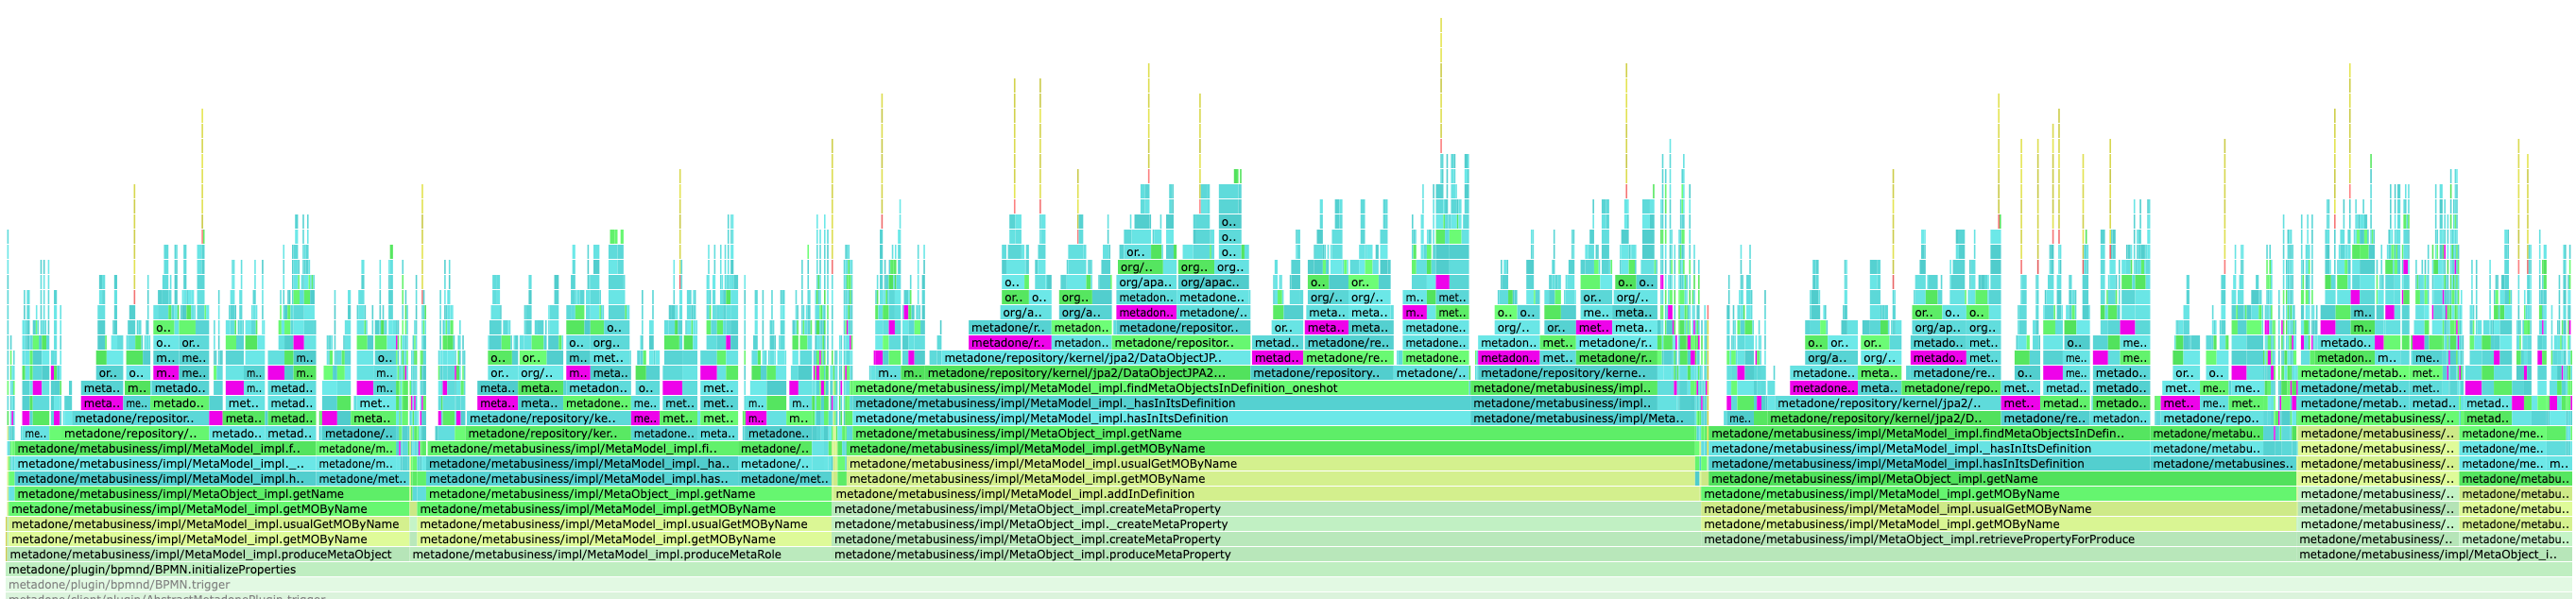
\includegraphics[width=\textwidth]{img/scenario1/prof1/check.png}
    \caption{\texttt{check} ---
    bundle \texttt{metadone\_bundle\_repository\_jpa2}}
\end{subfigure}

\medskip
\begin{subfigure}{\textwidth}
    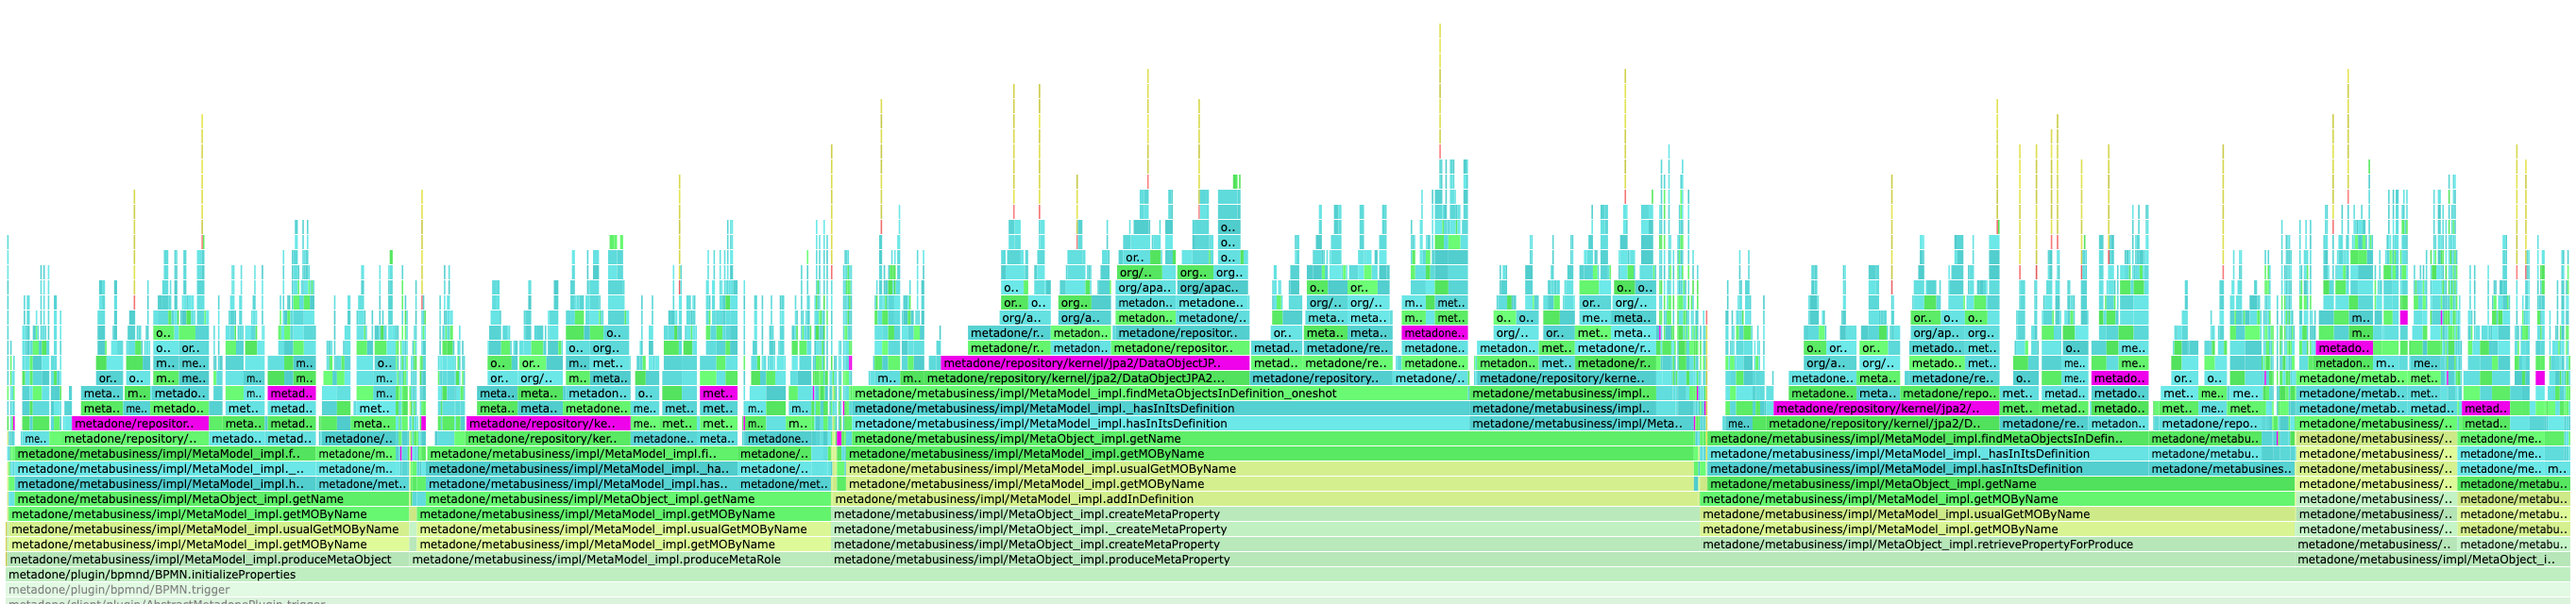
\includegraphics[width=\textwidth]{img/scenario1/prof1/getModel.png}
    \caption{\texttt{getModel} ---
    bundle \texttt{metadone\_bundle\_repository\_jpa2}}
\end{subfigure}

\medskip
\begin{subfigure}{\textwidth}
    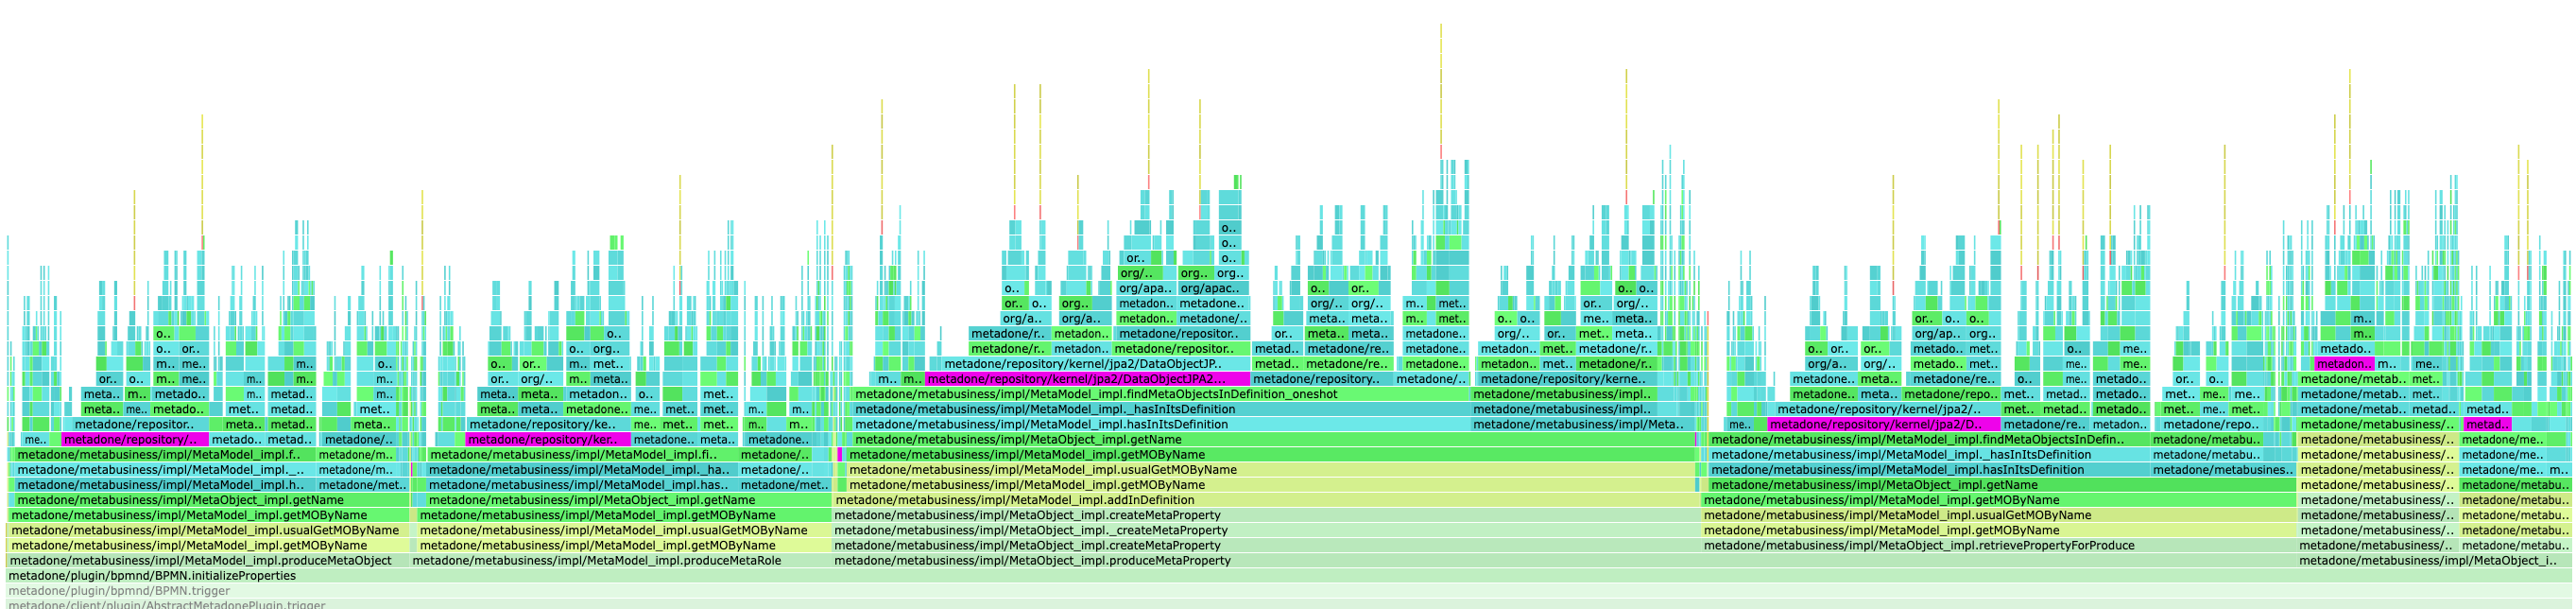
\includegraphics[width=\textwidth]{img/scenario1/prof1/getRangeOf.png}
    \caption{\texttt{getRangeOf} --- 
    bundle \texttt{metadone\_bundle\_repository}}
\end{subfigure}

\medskip
\begin{subfigure}{\textwidth}
    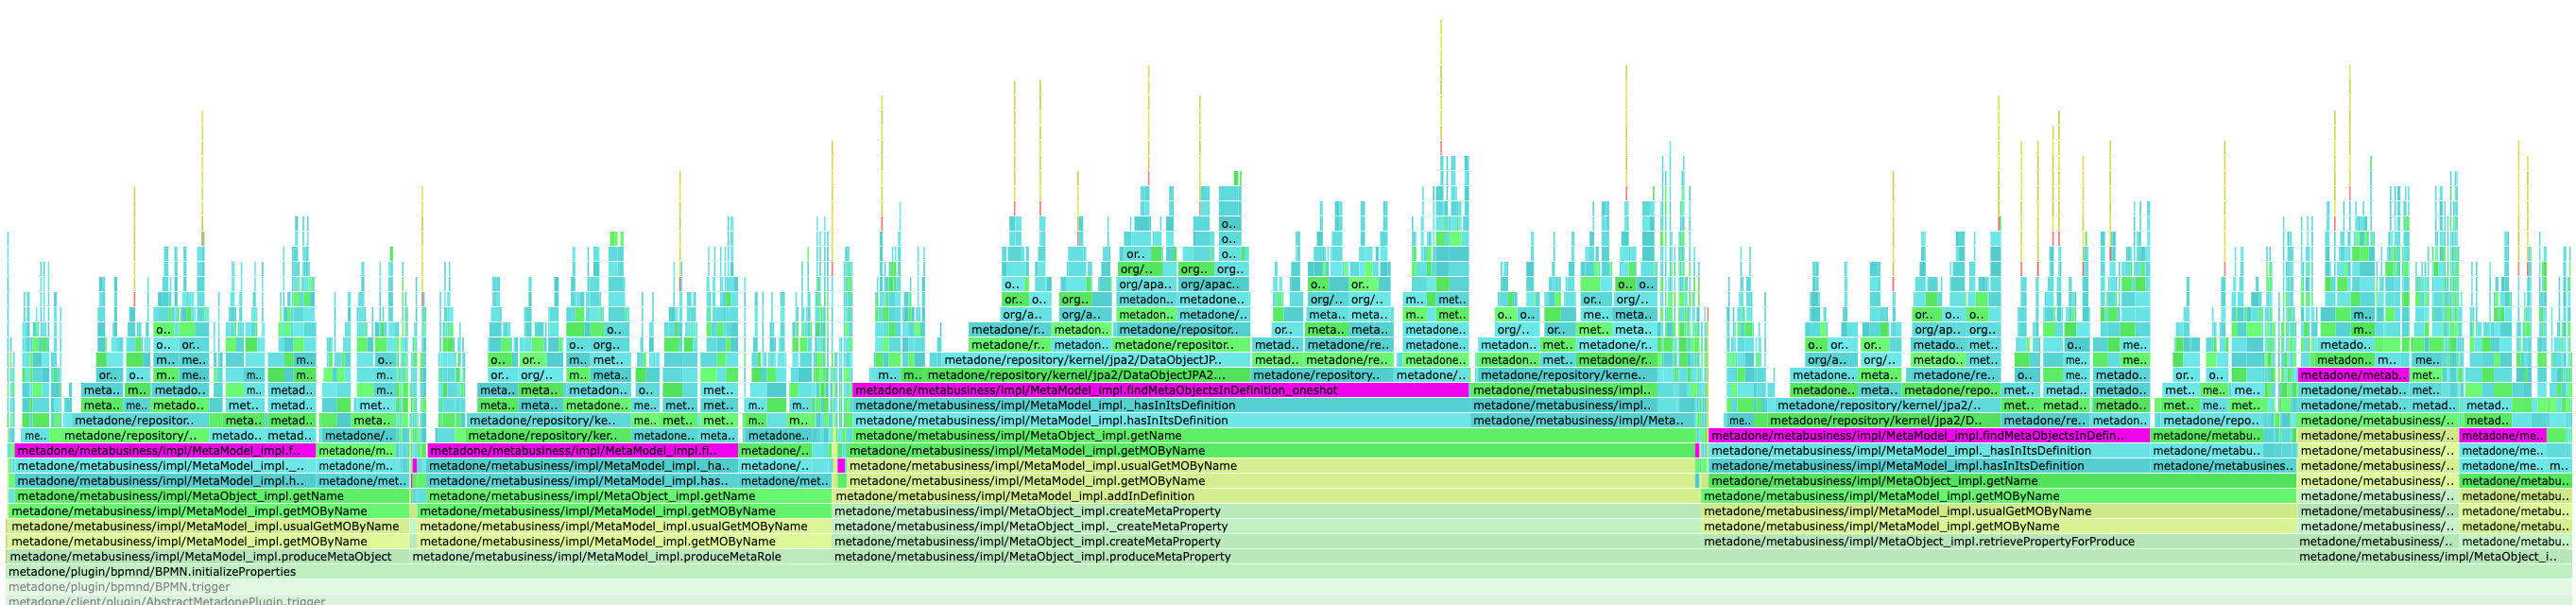
\includegraphics[width=\textwidth]{img/scenario1/prof1/oneshot.png}
    \caption{\texttt{findMetaObjectsInDefinition\_oneshot} --- classe \texttt{MetaModel\_impl}, bundle \texttt{metadone\_bundle\_metabusiness}}
\end{subfigure}

\caption{Flamegraphs isolant la phase d'initialisation du plugin BPMN.}
\label{fig:prof1-zoom}
\end{figure}

Le flamegraph révèle que \texttt{findMetaObjectsInDefinition\_oneshot} est
la méthode terminale d'une pile d'appels extrêmement coûteuse, représentant
plus de 56\% de l'utilisation CPU sur cette phase.

% -----------------------------------------------
\subsubsection{Analyse statique du code et quantification des appels}
% -----------------------------------------------

Afin de confirmer le diagnostic du profilage, nous avons procédé à une
analyse statique du code source couplée à une instrumentation manuelle par
compteurs d'appels. Les mesures confirment une amplification significative~:
pour 1~400 exécutions de \texttt{\_hasInItsDefinition}
(\texttt{MetaModel\_impl}, bundle \texttt{metadone\_bundle\_metabusiness}),
on dénombre plus de 80~000 appels à
\texttt{findMetaObjectsInDefinition\_oneshot}, soit un \textbf{facteur
multiplicatif moyen de 57}.

La cause de cette amplification réside dans la structure de \texttt{\_hasInItsDefinition} (Listing~\ref{ls-has})~: chaque invocation appelle \texttt{findMetaObjectsInDefinition\_oneshot} pour le \texttt{MetaModel} courant (ligne 180), puis pour chacun de ses supertypes \texttt{MetaModel} (ligne 183), multipliant les invocations avec la profondeur de la hiérarchie. Cette hiérarchie est précisément rendue possible par la réflexivité de MetaL$_2$~: \texttt{MetaModel} étend \texttt{MetaObject} (section~\ref{sec:metal2}), si bien que les supertypes d'un \texttt{MetaModel} sont eux-mêmes des \texttt{MetaModel} et déclenchent à leur tour la récursion.

\begin{lstlisting}[firstnumber=174,
  caption={Méthode \texttt{\_hasInItsDefinition} ---
  classe \texttt{MetaModel\_impl},
  bundle \texttt{metadone\_bundle\_metabusiness}},
  label={ls-has}]
private boolean _hasInItsDefinition(MetaObject_impl mo) {
    try {
        final Set<MetaObject> found =
            cache_getMetaObjectsInDefinition
                .isCachedNotNull(mo.getTarget()
                    .getDataObject().getOID());
        if (found != null && found.contains(mo)) {
            return true;
        } else {
            if (this.findMetaObjectsInDefinition_oneshot(mo)) {
                return true;
            } else {
                for (final MetaObject supertype : getAllSupertypes()) {
                    if (supertype.isA(MetaModel.class)) {
                        final MetaModel_impl mm =
                            supertype.narrow(MetaModel_impl.class);
                        if (mm.findMetaObjectsInDefinition_oneshot(mo)) {
                            return true;
                        }
                    }
                }
            }
            return false;
        }
    } catch (final BadPreCondition e) {
        throw new Metal2Exception(e);
    }
}
\end{lstlisting}

La méthode \texttt{findMetaObjectsInDefinition\_oneshot}
(Listing~\ref{ls-oneshot}) répond à une question précise~: le
\texttt{MetaObject} \texttt{partSide} appartient-il directement à la
définition du \texttt{MetaModel} \texttt{this}~?

Pour le comprendre, il faut rappeler comment l'appartenance d'un \texttt{MetaObject} à un \texttt{MetaModel} est encodée dans le kernel~: lors de l'ajout d'un \texttt{MetaObject} à la définition d'un \texttt{MetaModel}, une \texttt{K\_PropertyType} de type \texttt{def\_pt} est créée, reliant le \texttt{MetaObject} (domaine)
au \texttt{MetaModel} (range). La méthode itère donc sur l'ensemble des
propriétés de type \texttt{def\_pt} dont le \texttt{MetaModel} courant est
le range (ligne 204) --- c'est-à-dire toutes les relations d'appartenance
pointant vers ce modèle --- et vérifie pour chacune que son domaine est le
\texttt{MetaObject} recherché (ligne 206). Il s'agit d'une \textbf{recherche
linéaire de complexité $O(n)$}, où $n$ est le nombre de \texttt{MetaObject}
dans la définition du \texttt{MetaModel} considéré.

Cette recherche repose sur \texttt{getRangeOf()} de l'interface
\texttt{K\_Object} (bundle \texttt{metadone\_bundle\_repository}), qui retourne la liste des propriétés dont
l'objet est le range~: c'est l'opération de traversée du graphe de
\texttt{DataObject} qui apparaît au bas du flamegraph et représente
29,33\% du CPU.

\begin{lstlisting}[firstnumber=199,
  caption={Méthode \texttt{findMetaObjectsInDefinition\_oneshot} ---
  classe \texttt{MetaModel\_impl},
  bundle \texttt{metadone\_bundle\_metabusiness}},
  label={ls-oneshot}]
private final boolean findMetaObjectsInDefinition_oneshot(
        MetaObject_impl partSide) {
    try {
        final K_ObjectType wholeSide = this.getTarget();
        final K_ObjectType partSide_o = partSide.getTarget();
        final K_PropertyType defIsDependentOf_pt =
            getWorkspace().getDefIsDependentOf_pt();
        for (final K_Property def_p :
                wholeSide.getRangeOf(workspace.getDef_pt())) {
            final K_Object def_o =
                def_p.getDataObject().narrow_K_Object();
            if (def_o != null &&
                    def_o.getDomainOfIter(defIsDependentOf_pt)
                        .hasNext()) {
                if (def_p.getDomain().equals(partSide_o)) {
                    return true;
                }
            }
        }
        return false;
    } catch (final BadFacet e) {
        throw new Metal2Exception(e);
    } catch (final BadPreCondition e) {
        throw new Metal2Exception(e);
    }
}
\end{lstlisting}

% -----------------------------------------------
\subsubsection{Synthèse du diagnostic}
% -----------------------------------------------

Le goulot d'étranglement ne provient pas d'un algorithme intrinsèquement
complexe, mais de l'accumulation de recherches linéaires répétées dans des
boucles imbriquées.
La pile d'appels problématique est la suivante~:

\begin{center}
\small
\texttt{MetaModel\_impl.\_hasInItsDefinition} \\
(itération sur les supertypes via \texttt{getAllSupertypes()}) \\[4pt]
$\downarrow$ \\[4pt]
\texttt{MetaModel\_impl.findMetaObjectsInDefinition\_oneshot} \\
(itération $O(n)$ sur les propriétés \texttt{def\_pt}) \\[4pt]
$\downarrow$ \\[4pt]
\texttt{K\_Object.getRangeOf} --- \texttt{metadone\_bundle\_repository} \\
(traversée du graphe de \texttt{DataObject}, 29,33\% CPU)
\end{center}

La mitigation naturelle est la \textbf{mémoïsation}~: si l'appartenance
d'un \texttt{MetaObject} à un \texttt{MetaModel} est déjà connue, la
traversée du graphe est superflue. Un mécanisme de cache existe dans le
code --- \texttt{cache\_getMetaObjectsInDefinition}, instance de
\texttt{CacheCallFunction} du bundle \texttt{metadone\_common} --- mais il est rendu inopérant par deux défauts cumulés~:

\begin{enumerate}
    \item \textbf{Cache désactivé à l'initialisation.} Le paramètre
    \texttt{false} passé au constructeur de \texttt{CacheCallFunction}
    désactive globalement le cache. Chaque appel à
    \texttt{\_hasInItsDefinition} court-circuite le cache et déclenche
    une traversée complète, quelle que soit la fréquence de la même
    requête.

    \item \textbf{Inversion de clé.} Lors de la consultation du cache,
    l'OID utilisé est celui du \texttt{MetaObject} recherché (\texttt{mo}),
    alors que le cache est indexé par OID de \texttt{MetaModel}
    (\texttt{this}). Même si le cache avait été activé, cette inversion
    garantissait une absence systématique de correspondance, rendant le
    cache indiscernable d'une absence totale.
\end{enumerate}

Ces deux défauts conjugués expliquent le facteur multiplicatif de 57
observé. La phase d'optimisation s'articulera autour de deux axes
complémentaires~: la correction du cache existant, et la substitution des
recherches linéaires par des structures d'accès en $O(1)$, présentés à la
section suivante.